\section{Datenspeicherung}
Als Speichermedium wird eine $\mu$SD-Karte verwendet, welche direkt in ein Breakoutboard gesteckt wird.\\
\subsection{Breakoutboard}
Das Breakoutboard (siehe Abb. \ref{fig:muSDBreakout}) kann wegen des intern implementierten \textit{CD74HC4050 high-speed logic level translators}\footnote{konvertiert eine high-level logik in eine low-level logik} mit 5V betrieben werden. Das Arduino Mega Board und das Breakoutboard werden über SPI (siehe Kapitel \ref{subsubsec:spi}) nach dem Master-Slave Kommunikationsprinzip miteinander verbunden. 
\begin{figure}[h]
\centering
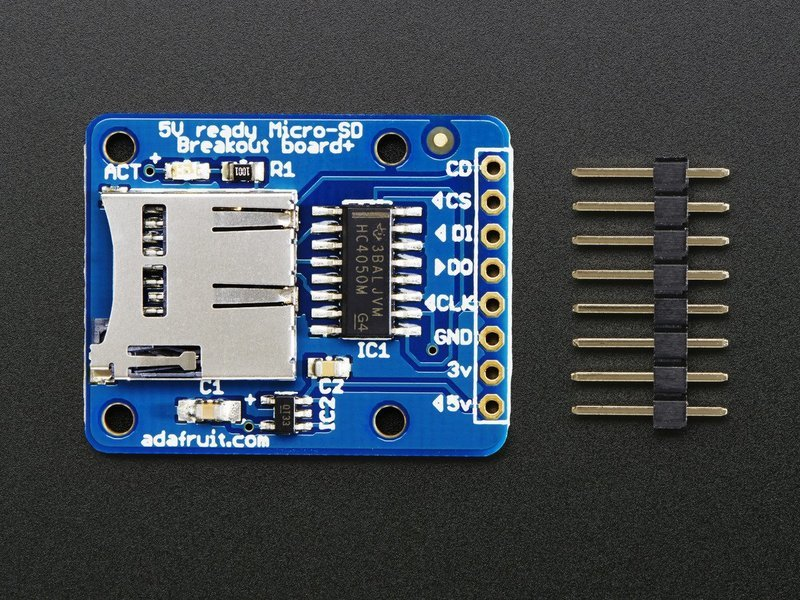
\includegraphics[width=0.5\linewidth]{graphics/Datenspeicherung/micro_sd_card_breakout.png}
\caption{254 $\mu$SD-Breakoutboard von Adafruit \cite{ladyada2018}}
\label{fig:muSDBreakout}
\end{figure}

\subsubsection{SPI (Serial Peripheral Interface)}
\label{subsubsec:spi}
\subsubsection{Verdrahtung}
SD-Karten erfordern viel Datenübertragung. Deshalb kann beste Leistung erbracht werden, wenn sie an die Hardware-SPI-Pins eines Mikrocontrollers angeschlossen werden. Dabei wird es wie folgt miteinander verbunden: \cite{ladyada2018}
\begin{itemize}
\item \textbf{5V} und \textbf{GND} Pins jeweils auf die \textbf{5V} und \textbf{GND} Pins des Arduino Mega Boards
\item \textbf{CLK} auf die Pinnummer \textbf{52}
\item \textbf{DO} auf die Pinnummer \textbf{50}
\item \textbf{DI} auf die Pinnummer \textbf{51}
\item \textbf{CS} auf die Pinnummer \textbf{53}
\end{itemize}

\subsection{$\mu$SD-Karte}
\begin{figure}[h]
\centering
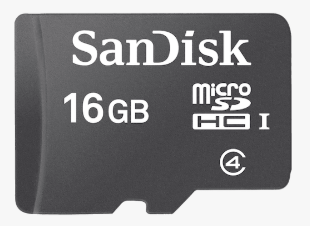
\includegraphics[width=0.2\linewidth]{graphics/Datenspeicherung/micro_sd_card_16GB.png}
\caption{16 GB $\mu$SD-Karte}
\label{fig:muSDKarte}
\end{figure}
